% Soubory musí být v kódování, které je nastaveno v příkazu \usepackage[...]{inputenc}

\documentclass[%
  12pt,       				% Velikost základního písma je 12 bodů
  a4paper,    				% Formát papíru je A4
  twoside,      			% Jednostranný tisk (výchozí)
	unicode,						% Záložky a informace budou v kódování unicode
  english,            % originální jazyk je angličtina
]{report}				    	% Dokument třídy 'zpráva'

\usepackage[utf8]		%	Kódování zdrojových souborů je v UTF-8
	{inputenc}					% Balíček pro nastavení kódování zdrojových souborů

\usepackage{graphicx} % Balíček 'graphicx' pro vkládání obrázků
											% Nutné pro vložení log školy a fakulty

\usepackage[
	nohyperlinks				% Nebudou tvořeny hypertextové odkazy do seznamu zkratek
]{acronym}						% Balíček 'acronym' pro sazby zkratek a symbolů
											% Nutné pro použití prostředí 'seznamzkratek' balíčku 'thesis'

\usepackage[
	breaklinks=true,		% Hypertextové odkazy mohou obsahovat zalomení řádku
	hypertexnames=false % Názvy hypertextových odkazů budou tvořeny
											% nezávisle na názvech TeXu
]{hyperref}						% Balíček 'hyperref' pro sazbu hypertextových odkazů
											% Nutné pro použití příkazu 'nastavenipdf' balíčku 'thesis'

\usepackage{pdfpages} % Balíček umožňující vkládat stránky z PDF souborů
                      % Nutné při vkládání titulních listů a zadání přímo
                      % ve formátu PDF z informačního systému

\usepackage{enumitem} % Balíček pro nastavení mezerování v odrážkách
  \setlist{topsep=0pt,partopsep=0pt,noitemsep}

\usepackage{cmap} 		% Balíček cmap zajišťuje, že PDF vytvořené `pdflatexem' je
											% plně "prohledávatelné" a "kopírovatelné"

\usepackage{upgreek}	% Balíček pro sazbu stojatých řeckých písmem
											% např. stojaté pí: \uppi
											% např. stojaté mí: \upmu (použitelné třeba v mikrometrech)
											% pozor, grafická nekompatibilita s fonty typu Computer Modern!

\usepackage{dirtree}		% sazba adresářové struktury

\usepackage[formats]{listings}	% Balíček pro sazbu zdrojových textů
\lstset{
%	Definice jazyka použitého ve výpisech
%    language=[LaTeX]{TeX},	% LaTeX
%	language={Matlab},		% Matlab
	language={C},           % jazyk C
    basicstyle=\ttfamily,	% definice základního stylu písma
    tabsize=2,			% definice velikosti tabulátoru
    inputencoding=utf8,         % pro soubory uložené v kódování UTF-8
    %inputencoding=cp1250,      % pro soubory uložené ve standardním kódování Windows CP1250
		columns=fixed,  %flexible,
		fontadjust=true %licovani sloupcu
    extendedchars=true,
    literate=%  definice symbolů s diakritikou
    {á}{{\'a}}1
    {č}{{\v{c}}}1
    {ď}{{\v{d}}}1
    {é}{{\'e}}1
    {ě}{{\v{e}}}1
    {í}{{\'i}}1
    {ň}{{\v{n}}}1
    {ó}{{\'o}}1
    {ř}{{\v{r}}}1
    {š}{{\v{s}}}1
    {ť}{{\v{t}}}1
    {ú}{{\'u}}1
    {ů}{{\r{u}}}1
    {ý}{{\'y}}1
    {ž}{{\v{z}}}1
    {Á}{{\'A}}1
    {Č}{{\v{C}}}1
    {Ď}{{\v{D}}}1
    {É}{{\'E}}1
    {Ě}{{\v{E}}}1
    {Í}{{\'I}}1
    {Ň}{{\v{N}}}1
    {Ó}{{\'O}}1
    {Ř}{{\v{R}}}1
    {Š}{{\v{S}}}1
    {Ť}{{\v{T}}}1
    {Ú}{{\'U}}1
    {Ů}{{\r{U}}}1
    {Ý}{{\'Y}}1
    {Ž}{{\v{Z}}}1
}

%% Nastavení českého jazyka při sazbě v češtině.
% Pro sazbu češtiny je možné použít mezinárodní balíček 'babel', jenž
% použití doporučujeme pro nové instalace (MikTeX2.8,TeXLive2009), nebo
% národní balíček 'czech', který doporučujeme ve starších instalacích.
% Balíček 'babel' bude správně fungovat pouze ve spojení s programy
% 'latex', 'pdflatex', zatímco balíček 'czech' bude fungovat ve spojení
% s programy 'cslatex', 'pdfcslatex'.
% Varianta A:
\usepackage
  {babel}             % Balíček pro sazbu různojazyčných dokumentů; kompilovat (pdf)latexem!
  										% převezme si z parametrů třídy správný jazyk
\usepackage{lmodern}	% vektorové fonty Latin Modern, nástupce půvoních Knuthových Computern Modern fontů
\usepackage{textcomp} % Dodatečné symboly
\usepackage[T1]{fontenc}  % Kódování fontu - mj. kvůli správným vzorům pro dělení slov
% Varianta B:
%\usepackage{czech}   % Alternativní balíček pro sazbu v českém jazyce, kompilovat (pdf)cslatexem!

\usepackage[%
  center,             % Rovnice a popisky plovoucich objektů budou zarovnány na střed (vychozi)
diploma						 % sazba diplomové práce
]{thesis}             % Balíček pro sazbu studentských prací
                      % Musí být vložen až jako poslední, aby
                      % ostatní balíčky nepřepisovaly jeho příkazy

%%%%%%%%%%%%%%%%%%%%%%%%%%%%%%%%%%%%%%%%%%%%%%%%%%%%%%%%%%%%%%%%%
%%%%%%      Definice informací o dokumentu             %%%%%%%%%%
%%%%%%%%%%%%%%%%%%%%%%%%%%%%%%%%%%%%%%%%%%%%%%%%%%%%%%%%%%%%%%%%%

%% Název práce:
\nazev{Image Recognition by Convolutional Neural Networks - Basic Concepts}
{Rozpoznávání obrazů konvolučními neuronovými sítěmi - základní koncepty}
% Jméno a příjmení autora ve tvaru
\autor[Bc.]{Ondřej}{Zapletal}

%% Jméno a příjmení vedoucího/školitele včetně titulů
\vedouci[Ing.]{Karel}{Horák}[Ph.D.]

%% Jméno a příjmení oponenta včetně titulů
%  [tituly před jménem]{Křestní}{Příjmení}[tituly za jménem]
% Pokud nemá titul za jménem, smažte celý řetězec '[...]'
% Uplatní se pouze v prezentaci k obhajobě;
% v případě, že nechcete, aby se na titulním snímku prezentace zobrazoval oponent, pouze jej zakomentujte;
% u obhajoby semestrální práce se oponent nezobrazuje
\oponent[doc.\ Mgr.]{Křestní}{Příjmení}[Ph.D.]

%% Označení oboru studia
\oborstudia{Cybernetics, Control and Measurements}{Kybernetika, automatizace a měření}
%% Označení fakulty
\fakulta{Faculty of Electrical Engineering and Communication}{Fakulta elektrotechniky a komunikačních technologií}

%% Označení ústavu
\ustav{Department of Control and Instrumentation}{Ústav automatizace a měřicí techniky}

\logofakulta[loga/FEKT_zkratka_barevne_PANTONE_CZ]{loga/UTKO_color_PANTONE_CZ}


%% Rok obhajoby
\rok{Rok}
\datum{1.\,1.\,1970} % Datum se uplatní pouze v prezentaci k obhajobě

%% Místo obhajoby
% Na titulních stránkách bude automaticky vysázeno VELKÝMI písmeny
\misto{Brno}

%% Abstrakt
\abstrakt{Abstrakt práce v~originálním jazyce
}{Překlad abstraktu v~angličtině (nebo češtině pokud je originální jazyk angličtina)
}

%% Klíčová slova
\klicovaslova{Klíčová slova v~originálním jazyce}%
	{Překlad klíčových slov v~angličtině nebo češtině}

%% Poděkování
\podekovanitext{Rád bych poděkoval vedoucímu diplomové práce panu Ing.~XXX YYY, Ph.D.\ za odborné vedení, konzultace, trpělivost a podnětné návrhy k~práci.}  % do tohoto souboru doplňte údaje o sobě, o názvu práce...

%%%%%%%%%%%%%%%%%%%%%%%%%%%%%%%%%%%%%%%%%%%%%%%%%%%%%%%%%%%%%%%%%%%%%%%%

%%%%%%%%%%%%%%%%%%%%%%%%%%%%%%%%%%%%%%%%%%%%%%%%%%%%%%%%%%%%%%%%%%%%%%%%
%%%%%%     Nastavení polí ve Vlastnostech dokumentu PDF      %%%%%%%%%%%
%%%%%%%%%%%%%%%%%%%%%%%%%%%%%%%%%%%%%%%%%%%%%%%%%%%%%%%%%%%%%%%%%%%%%%%%
%% Při vloženém balíčku 'hyperref' lze použít příkaz '\nastavenipdf'
\nastavenipdf
%%%%%%%%%%%%%%%%%%%%%%%%%%%%%%%%%%%%%%%%%%%%%%%%%%%%%%%%%%%%%%%%%%%%%%%

%%%%%%%%%%%%%%%%%%%%%%%%%%%%%%%%%%%%%%%%%%%%%%%%%%%%%%%%%%%%%%%%%%%%%%%
%%%%%%%%%%%       Začátek dokumentu               %%%%%%%%%%%%%%%%%%%%%
%%%%%%%%%%%%%%%%%%%%%%%%%%%%%%%%%%%%%%%%%%%%%%%%%%%%%%%%%%%%%%%%%%%%%%%
\begin{document}


%% Vložení desek generovaných informačním systémem
\includepdf[pages=1,offset=15.4mm -1in]%
  {pdf/student-desky}% název souboru nesmí obsahovat mezery!
% nebo vytvoření desek z balíčku
%\vytvorobalku
\setcounter{page}{1} %resetovani citace stranek - desky se necisluji

%% Vložení titulního listu generovaného informačním systémem
\includepdf[pages=1,offset=15.4mm -1in]%
  {pdf/student-titulka}% název souboru nesmí obsahovat mezery!
% nebo vytvoření titulní stránky z balíčku
%\vytvortitulku

%% Vložení zadání generovaného informačním systémem
\includepdf[pages=1,offset=-12mm -1in]%
  {pdf/student-zadani}% název souboru nesmí obsahovat mezery!

% nebo lze vytvořit prázdný list příkazem ze šablony
%\stranka{}%
%	{\sffamily\Huge\centering ZDE VLOŽIT LIST ZADÁNÍ}%
%	{\sffamily\centering Z~důvodu správného číslování stránek}

%% Vysázení stránky s abstraktem
\vytvorabstrakt

%% Vysázení prohlaseni o samostatnosti
\vytvorprohlaseni

%% Vysázení poděkování
\vytvorpodekovani

%% Vysázení obsahu
\obsah

%% Vysázení seznamu obrázků
\seznamobrazku

%% Vysázení seznamu tabulek
\seznamtabulek

%% Vysázení seznamu výpisů
\lstlistoflistings

%% Vložení souboru 'text/uvod.tex' s úvodem
\chapter*{Úvod}
\phantomsection
\addcontentsline{toc}{chapter}{Úvod}


Úvod studentské práce, např\,\dots

Tato práce se věnuje oblasti \zk{zkDSP} (\zkratkatext{zkDSP}), zejména jevům, které nastanou při nedodržení Nyquistovy podmínky pro \zkratka{symfvz}.%
\footnote{Tato věta je pouze ukázkou použití příkazů pro sazbu zkratek.}

%% Vložení souboru 'text/reseni' s popisem reseni práce
\chapter[Teoretická část studentské práce]{Teoretická část studentské\\ práce}

Teoretické zázemí studentské práce vhodně rozdělené do částí.

(Struktura navržená v~této šabloně je nejhrubší možná, po konzultaci s~vedoucím je vhodné zvolit přiléhavější.)


%% Vložení souboru 'text/vysledky' s popisem vysledků práce
\chapter{Výsledky studentské práce}

Praktická část a výsledky studenstké práce vhodně rozdělené do částí.

\section{Programové řešení}
Lorem ipsum dolor sit amet, consectetuer adipiscing elit. Nulla pulvinar eleifend sem. Integer in sapien. Etiam sapien elit, consequat eget, tristique non, venenatis quis, ante. In laoreet, magna id viverra tincidunt, sem odio bibendum justo, vel imperdiet sapien wisi sed libero. Aliquam in lorem sit amet leo accumsan lacinia. Cum sociis natoque penatibus et magnis dis parturient montes, nascetur ridiculus mus. Duis sapien nunc, commodo et, interdum suscipit, sollicitudin et, dolor. Suspendisse sagittis ultrices augue. Nullam lectus justo, vulputate eget mollis sed, tempor sed magna. In convallis. Praesent id justo in neque elementum ultrices. Neque porro quisquam est, qui dolorem ipsum quia dolor sit amet, consectetur, adipisci velit, sed quia non numquam eius modi tempora incidunt ut labore et dolore magnam aliquam quaerat voluptatem. Phasellus enim erat, vestibulum vel, aliquam a, posuere eu, velit. Aliquam erat volutpat. Nullam faucibus mi quis velit \cite{sr02/2009}.

Aliquam erat volutpat. Quisque porta. Integer imperdiet lectus quis justo. Nullam justo enim, consectetuer nec, ullamcorper ac, vestibulum in, elit. Nullam faucibus mi quis velit. Fusce tellus. Fusce consectetuer risus a nunc. Cras pede libero, dapibus nec, pretium sit amet, tempor quis. Morbi imperdiet, mauris ac auctor dictum, nisl ligula egestas nulla, et sollicitudin sem purus in lacus
\cite{CSN_ISO_690-2011,CSN_ISO_7144-1997,CSN_ISO_31-11}.
Mauris elementum mauris vitae tortor. Neque porro quisquam est, qui dolorem ipsum quia dolor sit amet, consectetur, adipisci velit, sed quia non numquam eius modi tempora incidunt ut labore et dolore magnam aliquam quaerat voluptatem. Quisque porta. Integer vulputate sem a nibh rutrum consequat. Nulla pulvinar eleifend sem. Praesent id justo in neque elementum ultrices \cite{BiernatovaSkupa2011:CSNISO690komentar}.

\section{Výsledky měření}
Fusce tellus odio, dapibus id fermentum quis, suscipit id erat. Fusce tellus. Morbi scelerisque luctus velit. In laoreet, magna id viverra tincidunt, sem odio bibendum justo, vel imperdiet sapien wisi sed libero. Quisque porta. Fusce suscipit libero eget elit. Nulla non lectus sed nisl molestie malesuada. Phasellus faucibus molestie nisl. Integer vulputate sem a nibh rutrum consequat. Proin mattis lacinia justo. Phasellus et lorem id felis nonummy placerat. Etiam ligula pede, sagittis quis, interdum ultricies, scelerisque eu. Cras elementum. Aenean placerat. Donec ipsum massa, ullamcorper in, auctor et, scelerisque sed, est. Aliquam ante. Integer imperdiet lectus quis justo. Vivamus ac leo pretium faucibus. Nullam faucibus mi quis velit.

Etiam quis quam. Neque porro quisquam est, qui dolorem ipsum quia dolor sit amet, consectetur, adipisci velit, sed quia non numquam eius modi tempora incidunt ut labore et dolore magnam aliquam quaerat voluptatem. Aliquam erat volutpat. Lorem ipsum dolor sit amet, consectetuer adipiscing elit \cite{sr02/2009,pravidla}. Nunc auctor. Neque porro quisquam est, qui dolorem ipsum quia dolor sit amet, consectetur, adipisci velit, sed quia non numquam eius modi tempora incidunt ut labore et dolore magnam aliquam quaerat voluptatem. Maecenas lorem. Maecenas libero. In laoreet, magna id viverra tincidunt, sem odio bibendum justo, vel imperdiet sapien wisi sed libero. Nullam rhoncus aliquam metus.

Integer rutrum, orci vestibulum ullamcorper ultricies, lacus quam ultricies odio, vitae placerat pede sem sit amet enim. Ut enim ad minim veniam, quis nostrud exercitation ullamco laboris nisi ut aliquip ex ea commodo consequat. Fusce tellus odio, dapibus id fermentum quis, suscipit id erat. Nullam eget nisl. Nunc auctor. Etiam dui sem, fermentum vitae, sagittis id, malesuada in, quam. Fusce dui leo, imperdiet in, aliquam sit amet, feugiat eu, orci. Curabitur vitae diam non enim vestibulum interdum. Aliquam erat volutpat. Pellentesque sapien. Phasellus enim erat, vestibulum vel, aliquam a, posuere eu, velit.

Fusce dui leo, imperdiet in, aliquam sit amet, feugiat eu, orci. Maecenas aliquet accumsan leo. Aliquam ornare wisi eu metus. Cum sociis natoque penatibus et magnis dis parturient montes, nascetur ridiculus mus. Aliquam erat volutpat. Donec iaculis gravida nulla. Sed elit dui, pellentesque a, faucibus vel, interdum nec, diam. Temporibus autem quibusdam et aut officiis debitis aut rerum necessitatibus saepe eveniet ut et voluptates repudiandae sint et molestiae non recusandae. Nulla non arcu lacinia neque faucibus fringilla. Phasellus enim erat, vestibulum vel, aliquam a, posuere eu, velit. Praesent vitae arcu tempor neque lacinia pretium
\cite{Walter1999,Svacina1999IEEE,RajmicSysel2002}.

Fusce suscipit libero eget elit. Integer vulputate sem a nibh rutrum consequat. Aliquam erat volutpat. Etiam neque. Nulla turpis magna, cursus sit amet, suscipit a, interdum id, felis. Nullam rhoncus aliquam metus. Etiam dui sem, fermentum vitae, sagittis id, malesuada in, quam. Nunc auctor. Nunc dapibus tortor vel mi dapibus sollicitudin. Praesent in mauris eu tortor porttitor accumsan. Nulla non arcu lacinia neque faucibus fringilla. Nullam lectus justo, vulputate eget mollis sed, tempor sed magna. Maecenas lorem. Aenean placerat. Donec vitae arcu. Maecenas lorem. Donec iaculis gravida nulla. Nulla non lectus sed nisl molestie malesuada.

Duis pulvinar. Nulla est. Duis condimentum augue id magna semper rutrum. Integer pellentesque quam vel velit. Aliquam ante. Nulla quis diam. Proin mattis lacinia justo. Aenean fermentum risus id tortor. Nunc auctor. Nullam justo enim, consectetuer nec, ullamcorper ac, vestibulum in, elit. In dapibus augue non sapien. Etiam bibendum elit eget erat. In sem justo, commodo ut, suscipit at, pharetra vitae, orci. Maecenas libero.

Nulla non lectus sed nisl molestie malesuada. Donec vitae arcu. Aenean fermentum risus id tortor. Praesent in mauris eu tortor porttitor accumsan. Nulla pulvinar eleifend sem. Duis viverra diam non justo. Integer imperdiet lectus quis justo. Pellentesque habitant morbi tristique senectus et netus et malesuada fames ac turpis egestas. In rutrum. Excepteur sint occaecat cupidatat non proident, sunt in culpa qui officia deserunt mollit anim id est laborum. Nulla non lectus sed nisl molestie malesuada. Aliquam erat volutpat. Mauris tincidunt sem sed arcu. Duis bibendum, lectus ut viverra rhoncus, dolor nunc faucibus libero, eget facilisis enim ipsum id lacus. Fusce tellus odio, dapibus id fermentum quis, suscipit id erat. In enim a arcu imperdiet malesuada. Nulla non lectus sed nisl molestie malesuada. Proin mattis lacinia justo.


%Pellentesque pretium lectus id turpis. Nemo enim ipsam voluptatem quia voluptas sit aspernatur aut odit aut fugit, sed quia consequuntur magni dolores eos qui ratione voluptatem sequi nesciunt. Curabitur ligula sapien, pulvinar a vestibulum quis, facilisis vel sapien. Praesent dapibus. Sed elit dui, pellentesque a, faucibus vel, interdum nec, diam. Duis viverra diam non justo. Duis ante orci, molestie vitae vehicula venenatis, tincidunt ac pede. Phasellus rhoncus. Maecenas fermentum, sem in pharetra pellentesque, velit turpis volutpat ante, in pharetra metus odio a lectus. Proin pede metus, vulputate nec, fermentum fringilla, vehicula vitae, justo. Fusce aliquam vestibulum ipsum. Nullam at arcu a est sollicitudin euismod.
%
%Aliquam ante. Phasellus faucibus molestie nisl. Etiam ligula pede, sagittis quis, interdum ultricies, scelerisque eu. Morbi leo mi, nonummy eget tristique non, rhoncus non leo. Cum sociis natoque penatibus et magnis dis parturient montes, nascetur ridiculus mus. Morbi scelerisque luctus velit. Curabitur bibendum justo non orci. Donec quis nibh at felis congue commodo. Nullam faucibus mi quis velit. Aenean id metus id velit ullamcorper pulvinar. Pellentesque sapien. Fusce nibh. Vestibulum fermentum tortor id mi. Nullam eget nisl. Praesent vitae arcu tempor neque lacinia pretium. Proin in tellus sit amet nibh dignissim sagittis. Donec quis nibh at felis congue commodo.
%
%Nam quis nulla. Proin in tellus sit amet nibh dignissim sagittis. Nullam dapibus fermentum ipsum. Curabitur ligula sapien, pulvinar a vestibulum quis, facilisis vel sapien. Nam libero tempore, cum soluta nobis est eligendi optio cumque nihil impedit quo minus id quod maxime placeat facere possimus, omnis voluptas assumenda est, omnis dolor repellendus. Vivamus ac leo pretium faucibus. Nunc tincidunt ante vitae massa. Maecenas sollicitudin. Ut tempus purus at lorem. Nullam lectus justo, vulputate eget mollis sed, tempor sed magna. Fusce consectetuer risus a nunc. Etiam quis quam.
%
%Donec quis nibh at felis congue commodo. Sed vel lectus. Donec odio tempus molestie, porttitor ut, iaculis quis, sem. Nullam feugiat, turpis at pulvinar vulputate, erat libero tristique tellus, nec bibendum odio risus sit amet ante. Sed elit dui, pellentesque a, faucibus vel, interdum nec, diam. Cras elementum. Sed vel lectus. Donec odio tempus molestie, porttitor ut, iaculis quis, sem. Etiam neque. Integer tempor. Vivamus porttitor turpis ac leo. Nulla non arcu lacinia neque faucibus fringilla.
%
%Etiam posuere lacus quis dolor. Nemo enim ipsam voluptatem quia voluptas sit aspernatur aut odit aut fugit, sed quia consequuntur magni dolores eos qui ratione voluptatem sequi nesciunt. Nullam faucibus mi quis velit. Cum sociis natoque penatibus et magnis dis parturient montes, nascetur ridiculus mus. Phasellus faucibus molestie nisl. Maecenas ipsum velit, consectetuer eu lobortis ut, dictum at dui. Maecenas aliquet accumsan leo. Pellentesque ipsum. Donec vitae arcu. Suspendisse nisl. Morbi imperdiet, mauris ac auctor dictum, nisl ligula egestas nulla, et sollicitudin sem purus in lacus. Pellentesque ipsum. Ut enim ad minima veniam, quis nostrum exercitationem ullam corporis suscipit laboriosam, nisi ut aliquid ex ea commodi consequatur? Nam libero tempore, cum soluta nobis est eligendi optio cumque nihil impedit quo minus id quod maxime placeat facere possimus, omnis voluptas assumenda est, omnis dolor repellendus.


%% Vložení souboru 'text/zaver' se závěrem
\chapter{Závěr}

Shrnutí studentské práce.


%% Vložení souboru 'text/literatura' se seznamem literatury
% Pro sazbu seznamu literatury použijte jednu z následujících možností

%%%%%%%%%%%%%%%%%%%%%%%%%%%%%%%%%%%%%%%%%%%%%%%%%%%%%%%%%%%%%%%%%%%%%%%%%
%1) Seznam citací definovaný přímo pomocí prostředí literatura / thebibliography

\begin{literatura}{99}
	
\bibitem{sr02/2009}
		VUT v~Brně:
    \emph{Úprava, odevzdávání a zveřejňování vysokoškolských kva\-li\-fi\-kač\-ních prací na VUT v~Brně}\/ [online].
		Směrnice rektora č.\,2/2009.
		Brno: 2009, po\-sled\-ní aktualizace 24.\,3.\,2009 [cit.\,23.\,10.\,2015].
    Dostupné z~URL:\\
    <\url{https://www.vutbr.cz/uredni-deska/vnitrni-predpisy-a-dokumenty/smernice-rektora-f34920/}>.

\bibitem{CSN_ISO_690-2011}
    \emph{ČSN ISO 690 (01 0197) Informace a dokumentace -- Pravidla pro bibliografické odkazy a citace informačních zdrojů.}
    40 stran. Praha: Český normalizační institut, 2011.

\bibitem{CSN_ISO_7144-1997}
    \emph{ČSN ISO 7144 (010161) Dokumentace -- Formální úprava disertací a podobných dokumentů.}
    24 stran. Praha: Český normalizační institut, 1997.

\bibitem{CSN_ISO_31-11}
    \emph{ČSN ISO 31-11 Veličiny a jednotky -- část 11: Matematické znaky a značky používané ve fyzikálních vědách a v~technice.}
    Praha: Český normalizační institut, 1999.

\bibitem{BiernatovaSkupa2011:CSNISO690komentar}
    BIERNÁTOVÁ, O., SKŮPA, J.:
    \emph{Bibliografické odkazy a citace dokumentů dle ČSN ISO 690 (01 0197) platné od 1.\,dubna 2011}\/ [online].
    2011, poslední aktualizace 2.\,9.\,2011 [cit. 19.\,10.\,2011].
    Dostupné z~URL:
    \(<\)\url{http://www.citace.com/CSN-ISO-690.pdf}\(>\)
%    \(<\)\href{http://www.boldis.cz/citace/citace.html}{http://www.boldis.cz/citace/citace.html}\(>\).

\bibitem{pravidla}
    \emph{Pravidla českého pravopisu}.
    Zpracoval kolektiv autorů. 1.\ vydání.
    Olomouc: FIN PUB\-LISH\-ING, 1998. 575 s. ISBN 80-86002-40-3.

\bibitem{Walter1999}
	WALTER, G.\,G.; SHEN, X.
	\emph{Wavelets and Other Orthogonal Systems}.
	2. vyd. Boca Raton: Chapman\,\&\,Hall/CRC, 2000. 392~s. ISBN 1-58488-227-1

\bibitem{Svacina1999IEEE}
	SVAČINA, J.
	Dispersion Characteristics of Multilayered Slotlines -- a Simple Approach.
	\emph{IEEE Transactions on Microwave Theory and Techniques},
	1999, vol.\,47, no.\,9, s.\,1826--1829. ISSN 0018-9480.

\bibitem{RajmicSysel2002}
    RAJMIC, P.; SYSEL, P.
    Wavelet Spectrum Thresholding Rules.
    In \emph{Proceedings of the International Conference Research in Telecommunication Technology},
    Žilina: Žilina University, 2002. s.\,60--63. ISBN 80-7100-991-1.

\end{literatura}


%%%%%%%%%%%%%%%%%%%%%%%%%%%%%%%%%%%%%%%%%%%%%%%%%%%%%%%%%%%%%%%%%%%%%%%%%
%%2) Seznam citací pomocí BibTeXu
%% Při použití je nutné v TeXnicCenter ve výstupním profilu aktivovat spouštění BibTeXu po překladu.
%% Definice stylu seznamu
%\bibliographystyle{unsrturl}
%% Pro českou sazbu lze použít styl czechiso.bst ze stránek
%% http://www.fit.vutbr.cz/~martinek/latex/czechiso.tar.gz
%%\bibliographystyle{czechiso}
%% Vložení souboru se seznamem citací
%\bibliography{text/literatura}
%
%% Následující příkaz je pouze pro ukázku sazby literatury při použití BibTeXu.
%% Způsobí citaci všech zdrojů v souboru odkazy.bib, i když nejsou citovány v textu.
%\nocite{*}

%% Vložení souboru 'text/zkratky' se seznam použitých symbolů, veličin a zkratek
\begin{seznamzkratek}{KolikMista}

	\novazkratka{zkTemp}		% název
		{Šířka levého sloupce Seznamu symbolů, veličin a zkratek}								% zkratka
		{je určena šířkou parametru prostředí \texttt{seznamzkratek} (viz řádek~1 výpisu zdrojáku na~str.\,\pageref{lst:zkratky})}
											% rozvinutí zkratky

	\novazkratka{zkDummy}
		{KolikMista}
		{pouze ukázka vyhrazeného místa}

	\novazkratka{zkDSP}		% název
		{DSP}								% zkratka
		{číslicové zpracování signálů -- Digital Signal Processing}
											% rozvinutí zkratky
	%%% bsymfvz
	\novazkratka{symfvz}						% název
		{\ensuremath{f_\textind{vz}}} % symbol
		{vzorkovací kmitočet}					% popis
	%%% esymfvz

\end{seznamzkratek}


%% Začátek příloh
\prilohy

%% Vysázení seznamu příloh
\seznampriloh

%% Vložení souboru 'text/prilohy' s přílohami
\chapter{Některé příkazy balíčku \texttt{thesis}}

\section{Příkazy pro sazbu veličin a jednotek}

\begin{table}[!h]
  \caption{Přehled příkazů pro matematické prostředí }
  \begin{center}
  	\small
	  \begin{tabular}{|c|c|c|c|}
	    \hline
	    Příkaz    						& Příklad 					& Zdroj příkladu  							& Význam  \\
	    \hline\hline
	    \verb|\textind{...}|	& $\beta_\textind{max}$ 	& \verb|$\beta_\textind{max}$|	& textový index \\
	    \hline
	    \verb|\konst{...}| 		& $\konst{U}_\textind{in}$ 				& \verb|$\konst{U}_\textind{in}$|		& konstantní veličina \\
	    \hline
	    \verb|\prom{...}| 		& $\prom{u}_\textind{in}$ & \verb|$\prom{u}_\textind{in}$| & proměnná veličina \\
	    \hline
	    \verb|\komplex{...}| 	& $\komplex{u}_\textind{in}$ & \verb|$\komplex{u}_\textind{in}$| & komplexní veličina \\
	    \hline
	    \verb|\vekt{...}| 		& $\vekt{y}$ 						& \verb|$\vekt{y}$| & vektor \\
	    \hline
	    \verb|\matice{...}| 	& $\matice{Z}$ 						& \verb|$\matice{Z}$| & matice \\
	    \hline
	    \verb|\jedn{...}| 		& $\jedn{kV}$ 						& \verb|$\jedn{kV}$|\quad či\ \, \verb|\jedn{kV}| & jednotka \\
	    \hline
	  \end{tabular}
  \end{center}
\end{table}



%\newpage
\section{Příkazy pro sazbu symbolů}

\begin{itemize}
  \item
    \verb|\E|, \verb|\eul| -- sazba Eulerova čísla: $\eul$,
  \item
    \verb|\J|, \verb|\jmag|, \verb|\I|, \verb|\imag| -- sazba imaginární jednotky: $\jmag$, $\imag$,
  \item
    \verb|\dif| -- sazba diferenciálu: $\dif$,
  \item
    \verb|\sinc| -- sazba funkce: $\sinc$.
  \item
    \verb|\mikro| -- sazba symbolu mikro stojatým písmem\footnote{znak pochází z~balíčku \texttt{textcomp}}: $\mikro$.

\end{itemize}
%
Všechny symboly jsou určeny pro matematický mód, vyjma \verb|\mikro|, jenž je\\ použitelný rovněž v~textovém módu.






\chapter{Druhá příloha}

\begin{figure}[!h]
  \begin{center}
    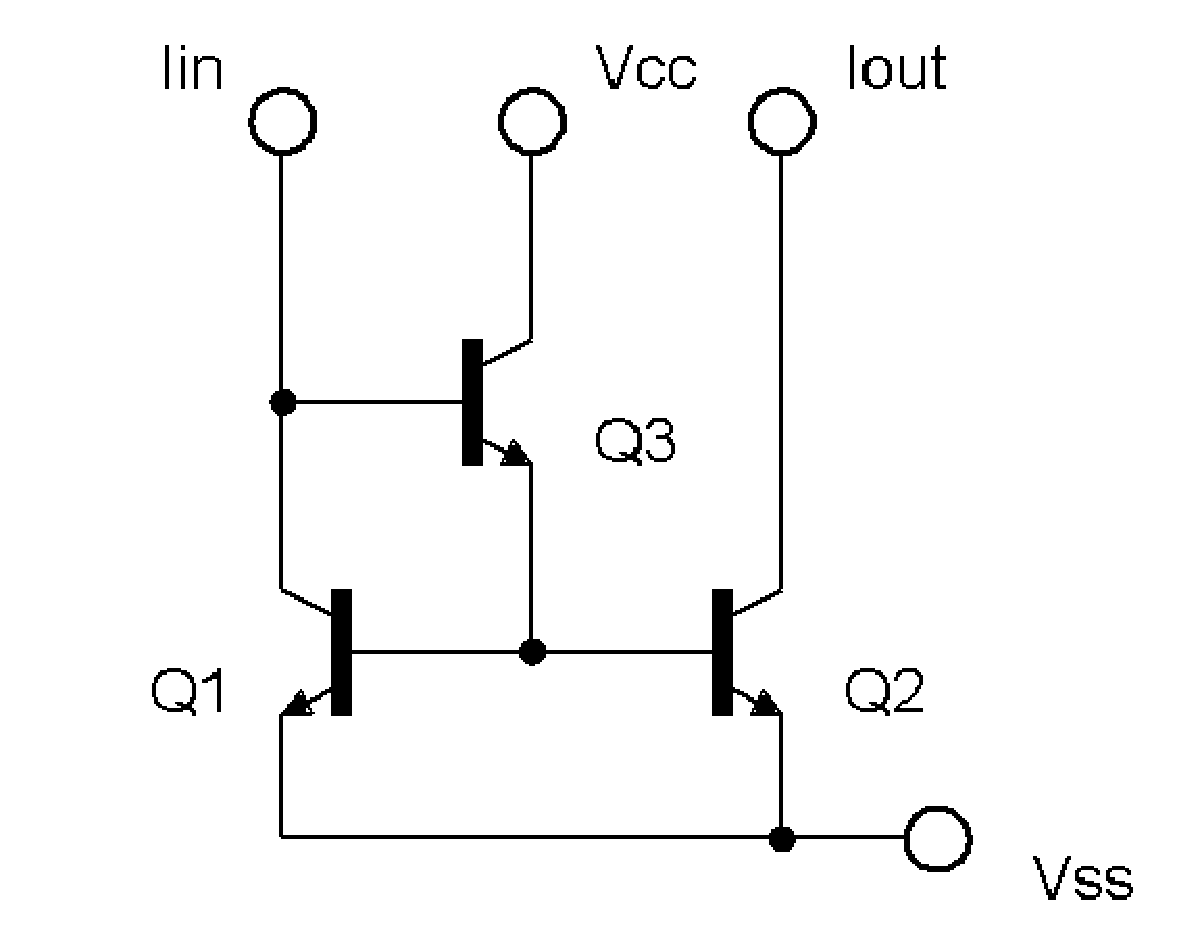
\includegraphics[scale=0.5]{obrazky/ZlepseneWilsonovoZrcadloNPN}
  \end{center}
  \caption{Zlepšené Wilsonovo proudové zrcadlo.}
\end{figure}

Pro sazbu vektorových obrázků přímo v~\LaTeX{}u je možné doporučit balíček \href{https://www.ctan.org/pkg/pgf}{\texttt{TikZ}}.
Příklady sazby je možné najít na \href{http://www.texample.net/tikz/examples/}{\TeX{}ample}.
Pro vyzkoušení je možné použít programy QTikz nebo TikzEdt.




\chapter{Příklad sazby zdrojových kódů}

\section{Balíček \texttt{listings}}

Pro vysázení zdrojových souborů je možné použít balíček \href{https://www.ctan.org/pkg/listings}{\texttt{listings}}.
Balíček zavádí nové prostředí \texttt{lstlisting} pro sazbu zdrojových kódů, jako například:
%
\begin{lstlisting}[language={[LaTeX]TeX}]
\section{Balíček lstlistings}
Pro vysázení zdrojových souborů je možné použít
	balíček \href{https://www.ctan.org/pkg/listings}%
	{\texttt{listings}}.
Balíček zavádí nové prostředí \texttt{lstlisting} pro
	sazbu zdrojových kódů.
\end{lstlisting}
%
Podporuje množství programovacích jazyků.
Kód k~vysázení může být načítán přímo ze zdrojových souborů.
Umožňuje vkládat čísla řádků nebo vypisovat jen vybrané úseky kódu.
Např.:

\noindent
Zkratky jsou sázeny v~prostředí \texttt{seznamzkratek}:
\label{lst:zkratky}
\lstinputlisting[language={[LaTeX]TeX},nolol,numbers=left,firstline=1,lastline=1]{text/zkratky.tex}
%
Šířka textu druhého parametru \verb|KolikMista| udává šířku prvního sloupce se zkratkami.
Proto by měla být zadávána nejdelší zkratka nebo symbol.
Příklad definice zkratky \zk{symfvz} je na výpisu \ref{lst:symfvz}.

\iflanguage{czech}{\shorthandoff{-}}{}
\iflanguage{slovak}{\shorthandoff{-}}{}
\lstinputlisting[language={[LaTeX]TeX},frame=single,caption={Ukázka sazby zkratek},label=lst:symfvz,numbers=left,linerange={bsymfvz-\%\%\%\ esymfvz},includerangemarker=false]{text/zkratky.tex}
\iflanguage{slovak}{\shorthandon{-}}{}
\iflanguage{czech}{\shorthandon{-}}{}

\noindent
Ukončení seznamu je provedeno ukončením prostředí:
\lstinputlisting[language={[LaTeX]TeX},nolol,numbers=left,firstnumber=22,linerange=22]{text/zkratky.tex}

\vspace{\fill}

\noindent
{\bf Poznámka k~výpisům s~použitím volby jazyka \verb|czech| nebo \verb|slovak|:}\newline
Pokud Váš zdrojový kód obsahuje znak spojovníku \verb|-|, pak překlad může skončit chybou.
Ta je způsobená tím, že znak \verb|-| je v~českém nebo slovenském nastavení balíčku \verb|babel| tzv.\ aktivním znakem.
Přepněte znak \verb|-| na neaktivní příkazem \verb|\shorthandoff{-}| těsně před výpisem a hned za ním jej vraťte na aktivní příkazem \verb|\shorthandon{-}|.
Podobně jako to je ukázáno ve zdrojovém kódu šablony.


\clearpage

%\section{Výpis kódu prostředí Matlab}
Na výpisu \ref{lst:priklad.vypis.kodu.Matlab} naleznete příklad kódu pro Matlab, na výpisu \ref{lst:priklad.vypis.kodu.C} zase pro jazyk~C.

\lstnewenvironment{matlab}[1][]{%
\iflanguage{czech}{\shorthandoff{-}}{}%
\iflanguage{slovak}{\shorthandoff{-}}{}%
\lstset{language=Matlab,numbers=left,#1}%
}{%
\iflanguage{slovak}{\shorthandon{-}}{}%
\iflanguage{czech}{\shorthandon{-}}{}%
}

\begin{matlab}[frame=single,float=htbp,caption={Příklad Schur-Cohnova testu stability v~prostředí Matlab.},label=lst:priklad.vypis.kodu.Matlab,numberstyle=\scriptsize, numbersep=7pt]
%% Priklad testovani stability filtru

% koeficienty polynomu ve jmenovateli
a = [ 5, 11.2, 5.44, -0.384, -2.3552, -1.2288];
disp( 'Polynom:'); disp(poly2str( a, 'z'))

disp('Kontrola pomoci korenu polynomu:');
zx = roots( a);
if( all( abs( zx) < 1))
    disp('System je stabilni')
else
    disp('System je nestabilni nebo na mezi stability');
end

disp(' '); disp('Kontrola pomoci Schur-Cohn:');
ma = zeros( length(a)-1,length(a));
ma(1,:) = a/a(1);
for( k = 1:length(a)-2)
    aa = ma(k,1:end-k+1);
    bb = fliplr( aa);
    ma(k+1,1:end-k+1) = (aa-aa(end)*bb)/(1-aa(end)^2);
end

if( all( abs( diag( ma.'))))
    disp('System je stabilni')
else
    disp('System je nestabilni nebo na mezi stability');
end
\end{matlab}

\noindent
\begin{minipage}{\linewidth}


%\section{Výpis kódu jazyka C}

\begin{lstlisting}[frame=single,numbers=right,caption={Příklad implementace první kanonické formy v~jazyce C.},label=lst:priklad.vypis.kodu.C,basicstyle=\ttfamily\small, keywordstyle=\color{black}\bfseries\underbar,]
// první kanonická forma
short fxdf2t( short coef[][5], short sample)
{
	static int v1[SECTIONS] = {0,0},v2[SECTIONS] = {0,0};
	int x, y, accu;
	short k;

	x = sample;
	for( k = 0; k < SECTIONS; k++){
		accu = v1[k] >> 1;
		y = _sadd( accu, _smpy( coef[k][0], x));
		y = _sshl(y, 1) >> 16;

		accu = v2[k] >> 1;
		accu = _sadd( accu, _smpy( coef[k][1], x));
		accu = _sadd( accu, _smpy( coef[k][2], y));
		v1[k] = _sshl( accu, 1);

		accu = _smpy( coef[k][3], x);
		accu = _sadd( accu, _smpy( coef[k][4], y));
		v2[k] = _sshl( accu, 1);

		x = y;
	}
	return( y);
}
\end{lstlisting}
\end{minipage}







\chapter{Obsah přiloženého CD}
Nezapomeňte uvést, co čtenář najde na přiloženém médiu.
Je vhodné okomentovat obsah každého adresáře, specifikovat, který soubor obsahuje důležitá nastavení, který soubor je určen ke spuštění atd.
Také je dobře napsat, v~jaké verzi software byl kód testován (např.\ Matlab 2010b).

Pokud je souborů hodně a jsou organizovány ve více složkách,  je možné pro výpis adresářové struktury použít balíček \href{https://www.ctan.org/pkg/dirtree}{\texttt{dirtree}}.

{\small
%
\dirtree{%.
.1 /\DTcomment{kořenový adresář přiloženého CD}.
.2 loga\DTcomment{loga školy a fakulty}.
.3 FEKT-spec-color.eps.
.3 FEKT-spec-color.pdf.
.3 logolink-op\_vavpi.png.
.3 RE-spec-color.eps.
.3 RE-spec-color.pdf.
.3 SIX\_logo\_zahlavi.png.
.2 obrazky\DTcomment{ostatní obrázky}.
.3 soucastky.eps.
.3 soucastky.png.
.3 spoje.eps.
.3 spoje.png.
.3 ZlepseneWilsonovoZrcadloNPN.eps.
.3 ZlepseneWilsonovoZrcadloNPN.png.
.3 ZlepseneWilsonovoZrcadloPNP.eps.
.3 ZlepseneWilsonovoZrcadloPNP.png.
.2 pdf\DTcomment{pdf stránky generované informačním systémem}.
.3 student-desky.pdf.
.3 student-titulka.pdf.
.3 student-zadani.pdf.
.2 text\DTcomment{zdrojové textové soubory}.
.3 literatura.tex.
.3 prilohy.tex.
.3 reseni.tex.
.3 uvod.tex.
.3 vysledky.tex.
.3 zaver.tex.
.3 zkratky.tex.
.2 navod-sablona\_FEKT.pdf\DTcomment{návod na používání šablony}.
.2 obhajoba.tex\DTcomment{hlavní soubor pro sazbu prezentace k~obhajobě}.
.2 readme.txt\DTcomment{soubor s~popisem obsahu CD}.
.2 sablona.tex\DTcomment{hlavní soubor pro sazbu kvalifikační práce}.
.2 thesis.sty\DTcomment{balíček pro sazbu kvalifikačních prací}.
}
}

%% Konec dokumentu
\end{document}
